\chapter{The Upgrade of the ITS}
%\lettrine{D} {$\mkern-\thinmuskip$}
During its first years of activity, the ALICE experiment has observed the creation of hot hadronic matter at unprecedented values of temperature and density, confirming the nature of the QGP as an almost-perfect fluid, as shown in previous experiments at BNL RHIC. Thanks to its unique tracking and PID capabilities, the measurements of the ALICE experiments exceeded the precision and kinematic reach of the QGP measures of its predecessors. However, it is still necessary to carry out high precision measurement of rare probes over a wide $\pt$ range, for which the current setup is not optimised.\\
In 2020, during the third run of data acquisition (Run3), the LHC will increase the luminosity of Pb-Pb collisions, reaching the interaction rate of 50 kHz, corresponding to an instantaneous luminosity of 6$\mathrm{\times 10^{27} cm^{-2}s^{-1}}$. The current collision rate is 8 kHz, while the readout rate of the detectors of the central barrel of the ALICE experiment is  0.5 - 1 kHz. For this reason, the current experimental set up does not allow to analyse all the Pb-Pb collisions provided by the LHC. For Run3, instead, the ALICE experiment will be upgraded to enable the readout of heavy-ion collisions at the rate of 50 kHz. Indeed, it is necessary to collect the data corresponding to all the Pb-Pb events, since for the objectives of the experiment no triggers are available. After the upgrade, more than 10 $\mathrm{nb^{-1}}$ of Pb-Pb collisions will be collected \cite{uptdr}. Among the detectors of the ALICE experiment, the Inner Tracking System will be replaced with a new detector. In this chapter, the upgraded ITS will be described, focusing on the physics motivations behind the upgrade, the layout of the new detector and the plans for the software development.
\section{Physics Motivations for the Upgrade}
One of the objectives of the upgrade is the study of heavy flavours, which are extremely important in heavy-ion physics since they are mainly produced in the first stages of the collision and, therefore, they allow to study the transport properties of the medium. There are two main questions related to the heavy-flavour interactions in the QGP:
\begin{itemize}
 \item the thermalization of heavy quarks in the medium, studying the baryon/ meson ratio for charm ($\Lambda_{c}$/D) and for beauty ($\Lambda_{b}$/B), the azimuthal anisotropy $v_2$ for charm mesons and baryons and possible in-medium thermal production of charm quarks.
 \item the heavy-quark in-medium energy loss and its mass dependence, which can be studied by measuring the nuclear modification factors $\RAA$ of $\pt$ distributions of D and B in a wide momentum range.
\end{itemize}
For all these measurements, it is necessary to reconstruct the open charm and beauty down to low transverse momentum ($\pt \leq$ 1 GeV/c) and to collect large statistics. The current configuration is not sufficient to fulfill these requests and an upgrade of the experimental setup is necessary. In particular, a larger statistics can be collected thanks to the higher collision rate, while the enhancement of the tracking resolution at low $\pt$ can be achieved with a low material budget.\\
Thanks to the reduced material budget and to the improved tracking precision and efficiency, it is possible to carry out a detailed measurement of low-mass dielectrons. These measurements are important because they give access not only to the thermal radiation from the QGP, of both real and virtual photons, but also to the in-medium modification of hadronic spectra related to chiral-symmetry restoration \cite{chiral}. Indeed, lattice QCD predicts that, at high temperatures, the restoration of chiral symmetry occurs, bringing some distortions in the vector and axial current spectra. This can empirically be seen as a change in the mass spectra, in particular for the meson $\rho$ in it $e^+e^-$ decay mode. This measurement implies the electron detection down to $\sim$ 100 MeV/c and, since the production rates of the thermal dileptons are low, a very good electron identification is needed to suppress combinatorial background, constituted primarily from $\pi^0$ Dalitz decays and photon conversions. For this reason, the upgraded experimental apparatus must be characterized by a low material budget before the first active layer. Moreover, good low-$\pt$ tracking capabilities are needed to track electrons down to $\pt \gtrsim $ 50 MeV/c, improving the reconstruction efficiency for the background suppression. Finally, by improving the secondary vertex resolution, it will be possible to discern electrons from semileptonic charm decays and to separate the charm contribution, allowing a better measurement of the thermal radiation.\\
The strong PID capabilities of the ALICE experiment are suitable for the spectroscopy of hypernuclei and exotic objects produced in Pb-Pb collisions. Hypernuclei are nuclei that contain at least a strange baryon (hyperon) in addition to protons and neutrons and their lifetime depend on the strength of the hyperon-nucleon interaction. The importance of such interactions is not only to describe the hadronic phase of a heavy-ion collision, but also to describe the hadronic matter in extreme density conditions, as for instance in neutron stars. In this context hyperon interactions are crucial to understand the phase structure of QCD at large densities. In particular, the mesonic decays of $^{3}_{\Lambda}$H , $^{4}_{\Lambda}$H  and $^{4}_{\Lambda}$He  are studied. The current data allows the detection of these states, but with a poor significance. Therefore, to improve the heavy-nuclear state analyses, the ALICE upgrade must fulfill two requirements: first, it must provide a larger statistics; then, it must improve the separation of the reconstructed signal decays from the combinatorial background, which can be obtained enhancing the tracking resolution. Besides the hypernuclei, more exotic forms of deeply bound states with strangeness have been proposed as states of matter, either consisting of baryons or quarks. Among these exotic objects, there are the H dibaryons, bound states of two $\Lambda$ mesons, and $\Lambda n$ bound states. These states have not been observed yet and hence, if they exist, are extremely rare. Moreover, the topology of their decay is very complex, making the detection efficiency low. Similarly to the case of hypernuclei, this analysis would benefit from the larger statistics and from a better tracking resolution.
\section{Layout of the ITS-Upgrade}
The readout rate of the current ITS is a strong limit: the readout times and the corresponding rate capabilities of the sub-detectors of the current ITS are reported in Table \ref{tab:curr}. These times depend only marginally on the detector occupancy and are very similar for pp and Pb-Pb collisions. The maximum rate of the current ITS is therefore about 1 kHz, with 100\% dead time, and constitutes a strict limit for the future physics studies. Moreover, the current configuration of the ITS is not sufficient for the study of heavy flavours. Indeed, heavy flavours are characterized by a short proper decay length ($c\tau$) and these values are low if compared to the current impact parameter resolution. In particular, the most abundantly produced charm baryon, the $\Lambda_{c}$, has a proper decay length of 60 $\mu m$, which is below the impact parameter resolution of the present ITS (see Figure \ref{fig:d0rphi}) in the transverse momentum range of the majority of the $\Lambda_{c}$ daughter particles. For this reason, the physics of charm baryons, along with that of beauty mesons and of beauty baryons, in not accessible with the current detector.\\
%
\begin{table}
\centering
\renewcommand\arraystretch{1.5}
 \begin{tabular}{|c|c|c|}
  \hline
  Sub-detector & Readout time ($\mu s$) & Rate (Hz)\\
  \hline
  SPD & 296 & 3300 \\
  SDD & 1023 & 985 \\
  SSD & 310 & 3265 \\
  \hline
 \end{tabular}
 \caption{Readout time of the current ITS sub-detectors and maximum rate capability.}
 \label{tab:curr}
\end{table}
%
In Run3 the current limitations will be overtaken with the complete substitution of the ITS. The ITS-Upgrade (ITSU) will consists of seven layers of sensors, to be compared with the six layers of the current configuration. The insertion of a further layer, closer to the interaction point, is possible thanks to the reduction of the size of the beam-pipe. The number and the radial positions of the layers have been determined considering the available space from the beam-pipe to the outer layer of the current ITS and studying, using Monte Carlo simulations, the disposition that optimizes the $\pt$ resolution in stand-alone mode.\\

\noindent
The key features of the ITSU, compared with the characteristics of the current ITS, will be briefly described in the following.
\begin{itemize}
 \item \textbf{First layer closer to the interaction point.}\\
 The current beam-pipe, with a radius of 29 mm, will be replaced with a new beam-pipe, with a radius of 19.2 mm. The thickness of the beam-pipe will remain 0.8 mm. Thanks to this change, in the upgrade layout the first active layer of the detector, which is currently positioned at 39 mm from the beam line,  will be positioned at 22.4 mm for the beam-line.
 \item \textbf{Reduction of the material budget.}\\
 The reduction of the material budget in the ITSU, in particular of the first active layer, is a key point in the improvement of the impact parameter resolution, enhancing the tracking performances and the momentum resolution. The improvement in the tracking resolution with the reduction of the material budget can be explained considering the Coulombian multiple-scattering formula \cite{pdg}:
 \begin{equation*}
  \theta_0 \; = \; \frac{13.6}{\beta c p } \: z \:  \sqrt{\frac{x}{X_0}} \: \left[1 + 0.038\ln\left(\frac{x}{X_0}\right)\right]
 \end{equation*}
 where $\theta_0$ is the angular dispersion, $\beta c$ is the speed of the charged particle, $p$ its momentum, $z$ its charge (expressed in terms of the elementary charge $e$), $x$ the thickness of the material and $X_0$ its radiation length. It is therefore clear that reducing the thickness of the material, the effects of the multiple scattering become smaller, allowing a better reconstruction of the trajectory of the particle. The reduction of the material budget will be achieved using \textit{Monolithic Silicon Pixel Sensors} (MAPS), passing form 200 $\mu m$ of the current SPD to 50 $\mu m$. MAPS will be describet more in detail later. Moreover, thanks to the optimisation of the readout chain, the power density is reduced of a factor of 2 if compared to the current sensors, allowing to increase the pixel density of a factor of 50. The lower consumption and the optimized power and signal distribution allow the reduction of the material budget of the electrical power and the signal cables. The final result is a detector with a thickness of 0.3\% $X_0$ for the three inner layers and of 0.8\%  $X_0$ for the outer layers.
 \item \textbf{Geometry and segmentation.}\\
 The ITSU will consist of seven layers of silicon pixels sensors. The three innermost layers form the \textit{Inner Barrel}, the remaining layers form the \textit{Outer Barrel}. The sensors of all the layers are segmented in pixels with dimensions of 20 $\times$ 20 $\mu m^2$. The layers are azimuthally segmented in units named \textit{Staves}, which are fixed to a support structure, half-wheel shaped, to form \textit{Half-Layers}. A single Stave consists of few elements:
 \begin{itemize}
  \item the \textit{Space Frame} is the mechanical support structure of the single stave, made of carbon fibre;
  \item the \textit{Cold Plate} is the carbon ply that embeds the cooling pipes;
  \item the \textit{Hybrid Integrated Circuit} is the flexible printed circuit (FPC) on which the Pixel Chips (two rows of seven sensors each) are bonded, along with passive components.
 \end{itemize}
 The Staves of the Outer Barrel are longitudinally segmented into \textit{Modules}, consisting of a Hybrid Integrated Circuit glued onto a carbon plate. Moreover, the Staves of the Outer Barrel are further segmented in azimuth in two halves, named \textit{Half-Staves}, which consist of a number of modules glued on a common cooling unit. The geometrical information about the ITSU is reported in Table \ref{tab:itsu}. 
 %
\begin{table}
\centering
\renewcommand\arraystretch{1.5}
 \begin{tabular}{|c|c|c|c|c|}
  \hline
  Layer & r (cm) & x/$X_0$ (\%) & \# sensors & \# staves\\
  \hline
  1 & 2.2 & 0.3 & 108 & 12\\
  2 & 3.0 & 0.3 & 144 & 16\\
  3 & 3.8 & 0.3 & 180 & 20\\
  4 & 19.4 & 0.8 & 2688 & 24\\
  5 & 24.4 & 0.8 & 3360 & 30\\
  6 & 34.2 & 0.8 & 8232 & 42\\
  7 & 39.2 & 0.8 & 9408 & 48\\
  \hline
 \end{tabular}
 \caption{Characteristics of the layers of the ITSU \cite{uptdr}.}
 \label{tab:itsu}
\end{table}
%
\begin{figure}
  \centering
  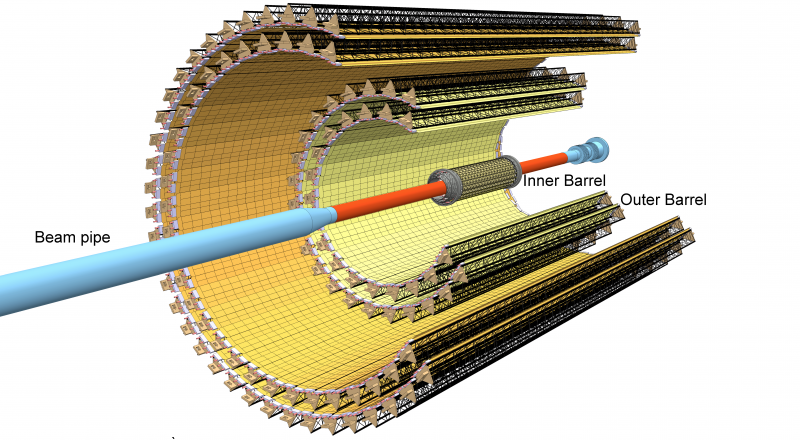
\includegraphics[scale=0.4]{figures/itsu.png}
  \caption{Layout of the upgraded Inner Tracking System.}
  \label{fig:build}
\end{figure}
%
\item \textbf{Binary readout}\\
In the ITSU there will be no analogue readout of the collected charge: each pixel has a single charge threshold and only the information whether a particle passed or not is available. Therefore, in the ITSU the particle identification via $dE/dx$ measurement will not be possible.
\item \textbf{Readout time}
The new detector is designed to be able to read data related to each individual interaction up to a rate of 100 kHz for Pb-Pb collisions and 400 kHz for pp collisions, a factor of 2 higher than the requirements. The new detector will support two different readout modes. 
In the \textit{continuous readout} mode, the information of the pixel matrices is shipped off-detector continuously, without a definition of event at readout level. The association of fired pixels to an event is done at the reconstruction level in the online system. In the \textit{trigger readout} mode, instead, only the fired pixels occurring in a particular time window that includes the event are shipped to the online system.
\end{itemize}
\section{MAPS}
\label{sec:maps}
Currently, the innermost layers of all the experiments of LHC are made of silicon pixel sensors bump-bonded on the readout electronics. Although this technology can be optimised, it has technical limitations that are close to be reached. For this reason, in the ITSU, Monolithic Active Pixel Sensors will be used: each pixel is monolithic, i.e. in the same piece of silicon both the active region and the readout electronics are present. In this way, it is possible to reduce the thickness of the sensors from the current value of 200 $\mu m$ for the SPD down to 50 $\mu m$. The working principle of a MAPS is shown in Figure \ref{fig:maps}. When a charge particle passes through the active volume of the silicon sensor, it liberates carriers in the semiconductor material. The released charge is collected by a sensing diode, which is a n-well normally used as a substrate of PMOS transistors. Consequently, only NMOS can be used in the pixel area, since a PMOS requires an additional n-well, which competes with the sensing diode in collecting the signal charge. Therefore, the front-end electronics fully relies on NMOS transistors and the n-wells that accommodate PMOS transistors are shielded by a deep p-well, which reflects the signal electrons so that they can be collected only by the sensing diode.
%
\begin{figure}
  \centering
  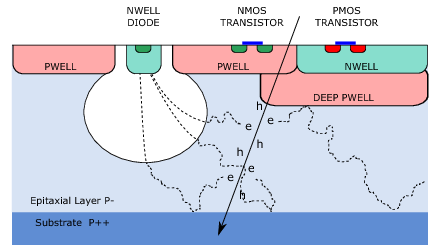
\includegraphics[scale=0.7]{figures/maps.png}
  \caption{Schematic cross section of a MAPS pixel \cite{uptdr}.}
  \label{fig:maps}
\end{figure}
%
The sensors must fulfill few requirements. First of all, they must have a low material budget and this condition is satisfied. Then, the performances of the ITSU and in particular its capabilities of separating secondary vertices of heavy-flavour decays is determined by the impact parameter resolution, which is enhanced thanks to the fine segmentation. Other important parameters for the track reconstruction are the detection efficiency, which must be at least 99\%, and the fake hit rate, which must be no more than $10^{-5}$. The performances of the sensors will be analysed later in this chapter.\\
Several prototypes of MAPS have been studied in the last years and the chosen one is ALPIDE (\textit{ALICE PIxel DEtector}), which is currently under development. This sensor has an active area of $15\times30 $ $mm^2$, corresponding to $512 \times 1024$ pixels with an extension of $20\times20$ $\mu m^2$ each. ALPIDE is characterized by a high-resistivity epitaxial layer (> 1 k$\Omega$), that allows a good charge collection. Its binary readout is performed with a combination of in-pixel discriminating frontend with a hit-driven combinatorial circuit. The former consists of a continuously active discriminating amplifier and a multiple-event memory in which the pixel information is stored. The memory is read out using a priority encoder, which takes into account only fired pixels: thanks to the low expected occupancy, the operation of pixel readout is fast \cite{alpide}.
\section{Detector Performances}
In this section the performances of the ITSU will be described. The results have been obtained using Monte Carlo simulations, with the geometrical parameters of the detectors previously described. The particle pseudorapidity-density has been extrapolated by the multiplicity measurements of Pb-Pb collision at $\sqrt{s_{NN}}$ = 2.76 TeV, obtaining a value of $dN_{ch}/d\eta \approx$ 1970 for central Pb-Pb collisions at $\sqrt{s_{NN}}$ = 5.5 TeV.
%
\begin{figure}
  \centering
  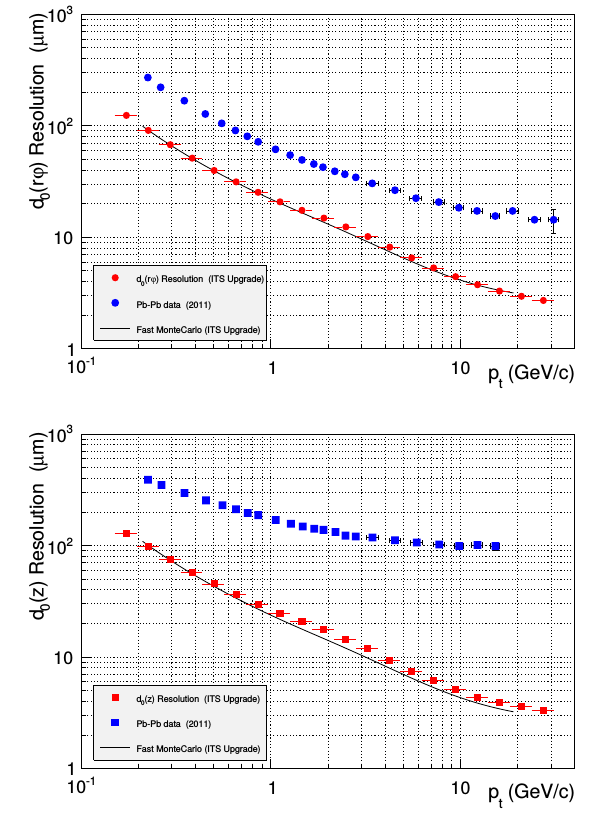
\includegraphics[scale=0.6]{figures/impactsim.png}
  \caption{Impact-parameter resolution for primary charged pions for the current ITS and for the ITSU in $r\varphi$ direction (upper panel) and $z$ direction (lower panel)\cite{uptdr}.}
  \label{fig:impactsim}
\end{figure}
%
The first important parameter is the impact-parameter resolution, since it defines the detector capability to discern the secondary vertex of heavy flavours from the primary vertex. This quantity is defined as the width of the distribution of the distances of closest approach between the reconstructed track and the interaction point. In Figure \ref{fig:impactsim} a simulation of the impact-parameter resolution for primary pions is shown together with the resolution in Pb-Pb data of the current detector. It is possible to see how the resolution will improve of a factor of 3 for $\pt$ < 1 GeV/c and of a factor of 5 for $\pt$ > 10 GeV/c.\\
%
\begin{figure}
  \centering
  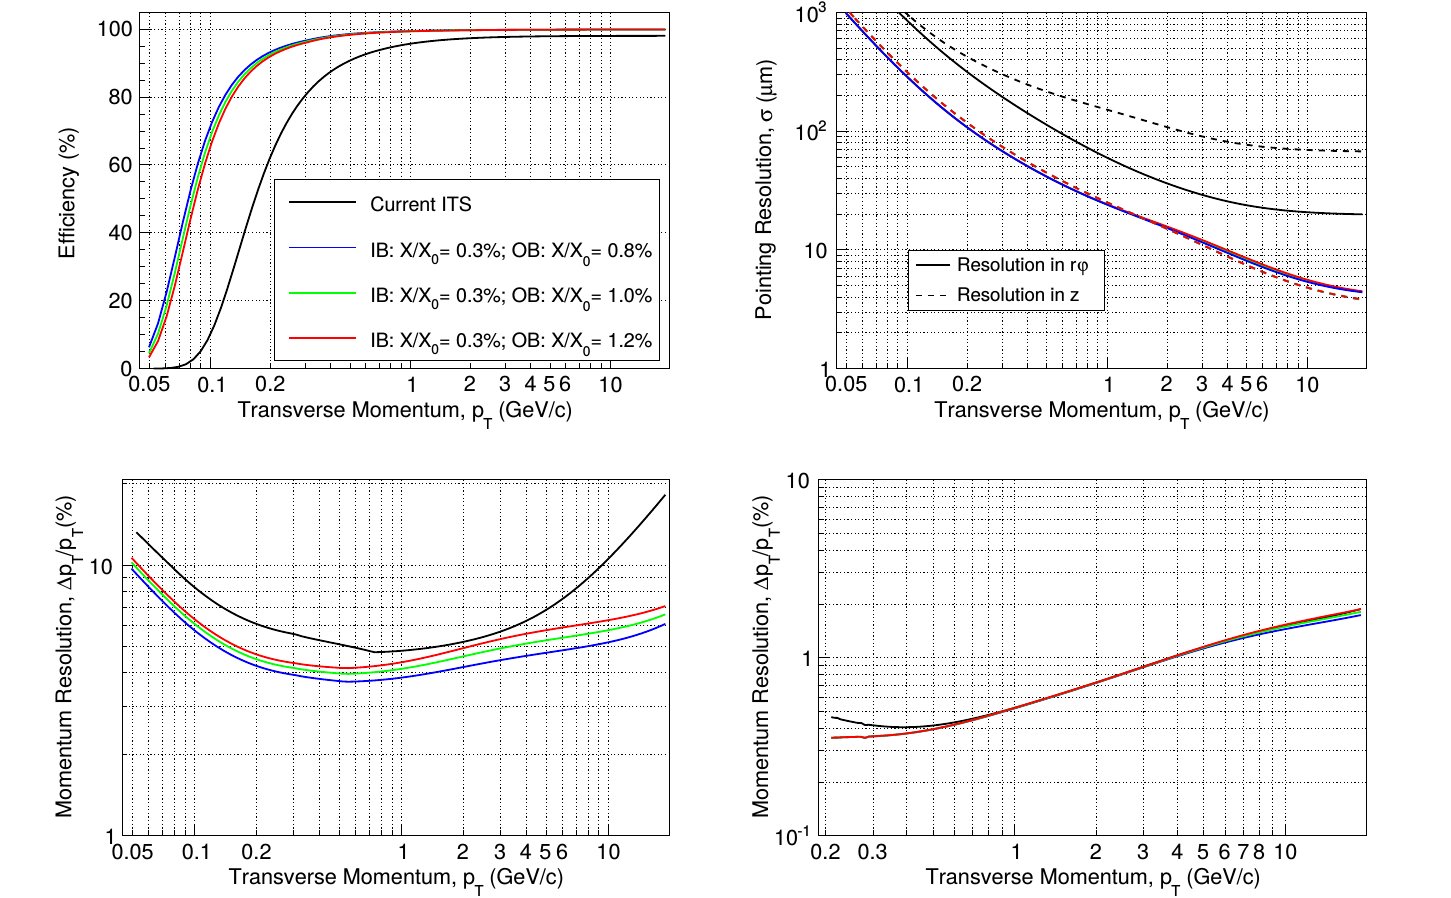
\includegraphics[scale=0.4]{figures/upperf.png}
  \caption{Stand-alone tracking efficiency (top-left panel) and pointing resolution (top-right panel) for charged pions of the current ITS and different material budget options for the ITSU. Transverse momentum resolution for charged pions for the current ITS and of the ITSU in stand-alone (bottom-left panel) and ITS+TPC (bottom-right panel) \cite{uptdr}.}
  \label{fig:upperf}
\end{figure}
%
In Figure \ref{fig:upperf} the results of the simulation for other important parameters of the upgraded detector are reported for different values of the material budget of the layers of the Outer Barrel. For the Inner Barrel a material budget of 0.3\% $X_0$ is always considered. The values are compared with the parameters of the current detector. Starting from the efficiency, there is not much difference between different values of material budget of the layers of the Outer Barrel, but in any case for each value of $\pt$ the efficiency is better. As far as the pointing resolution is concerned, its value will be better of about a factor of 5 in $r\varphi$ direction and of a factor of 20 in $z$ direction, due to the finest segmentation of the ITSU with respect to the current ITS.  The transverse momentum resolution in ITS stand-alone will improve with the upgrade and it is possible to notice how it is better for lower material budget of the outer layers. In ITS+TPC mode, instead, there is not much difference between different values of the material budget of the outer layers and, in general, an improvement is appreciable just for $\pt$ < 1 GeV/c.
\section{Physics Performances}
The heavy-flavour analysis is one of the fields that will benefit the most from the upgrade of the ITS. This is due to the better resolution of secondary vertices and impact parameters. In Figure \ref{fig:D0res} the case of the $D^0$ in the decay channel $D^0 \rightarrow K^-\pi^+$ is shown. In this figure the vertex resolutions for the current and the upgraded ITS, obtained via Monte Carlo simulations,  are reported. For the ITSU two kinds of simulations have been used: the \textit{full simulation} is a simulation completely based on the parameters of the upgraded detector, while the \textit{hybrid simulation} is based on existing Monte Carlo simulations for the current detector setup, scaled by the ratio between the resolution of the upgraded and the current detector as a function of $\pt$. It is possible to appreciate how the resolution of the secondary vertices improves of a factor of 3 in $x$ direction (and also in $y$ direction) and of a factor of 6 in $z$ direction. The consequence of this improvement in the vertex reconstruction is a better impact parameter resolution, which will improve of a factor of 3 with respect to the current ITS. Finally, from the previous consideration, the signal to noise ratio for the $D^0$ in the $D^0 \rightarrow K^-\pi^+$ decay channel can be estimated: for $\pt$ < 8 GeV/c there is an improvement of about a factor of 5, while for $\pt$ > 8 GeV/c it is better of a factor of 10 with respect to the current configuration. The two last comparisons can be seen in Figure \ref{fig:d0stuff}. This is just an example of how the measurement of heavy-flavours will benefit from the upgrade, but in general this improvement can be seen in all the D-meson measurements and also in B-meson measurements, since most of B-meson decay channels include a $D^0$ particle. Also the measurements of the heavy-flavour baryons will take advantage of the improved resolution and of the higher acquisition rate, i.e. higher statistics, that characterize the upgraded ITS.\\
The measurement of low-mass dielectrons in Pb-Pb collisions, not possible with the current detector, will be even more challenging, since there is the necessity to detect dileptons with an invariant mass down to $M_{ee} \approx 150$ MeV/$c^2$, that means to detect electrons with transverse momentum down to 100 - 200 MeV/c. This measurement is extremely difficult due to the huge combinatorial background, constituted of the electrons coming from $\pi^0$ Dalitz decays and from photon conversions. Thanks to the reduced material budget and the consequently enhanced low-$\pt$ tracking capability of the ITSU, it will be possible to track electrons down to $\pt \gtrsim $ 50 MeV/c, improving the reconstruction efficiency for those phenomena that form the combinatorial background.
%
\begin{figure}
  \centering
  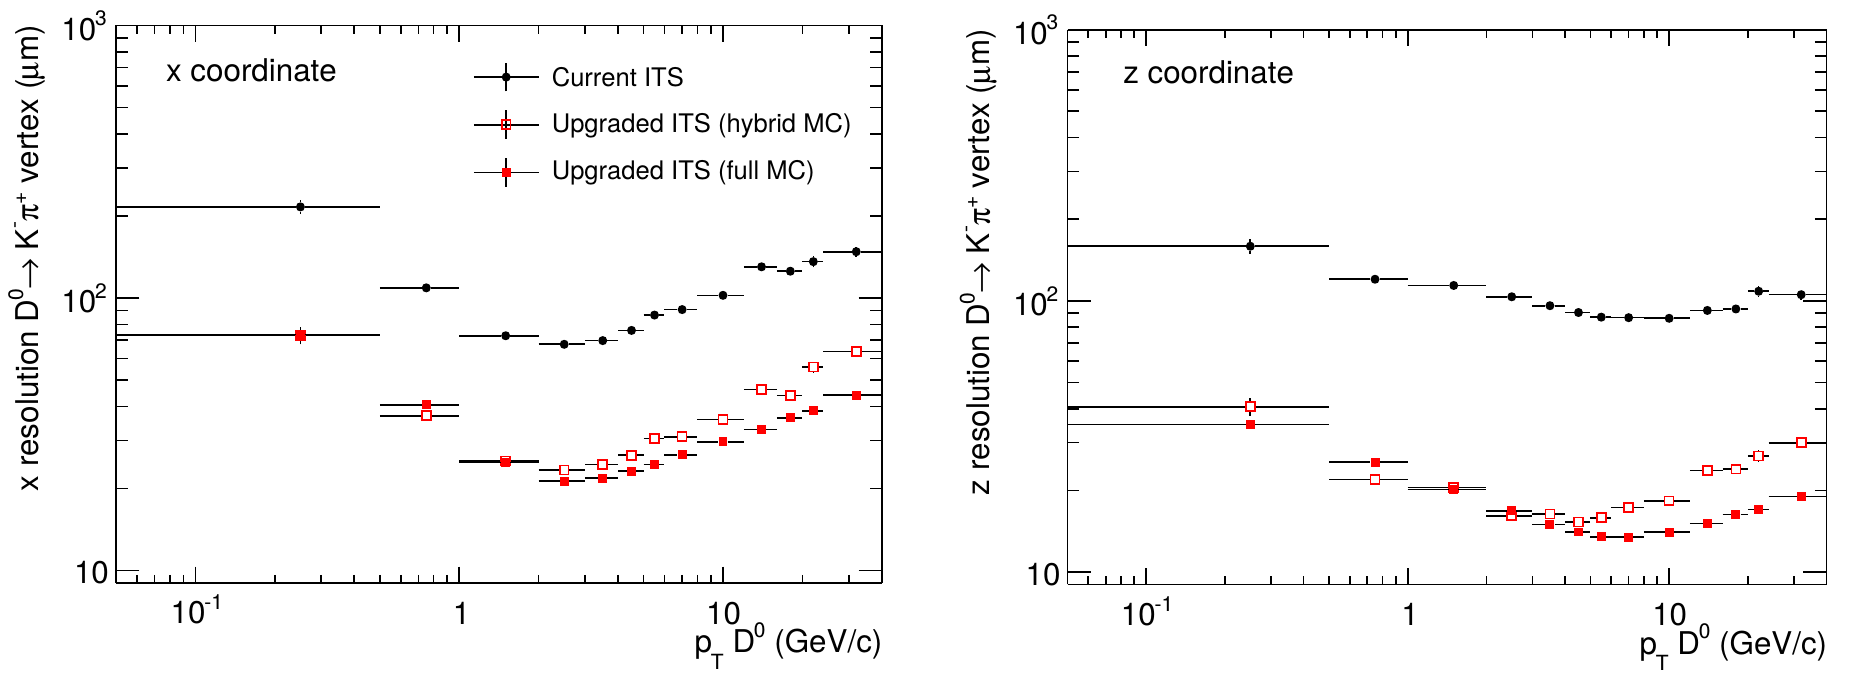
\includegraphics[scale=0.3]{figures/D0res.png}
  \caption{$D^0 \rightarrow K^-\pi^+$ secondary vertex position resolution for current and upgraded ITS in $x$ (left panel) and $z$ (right panel) \cite{uptdr}.}
  \label{fig:D0res}
  \vspace{1 cm}
  \centering
  {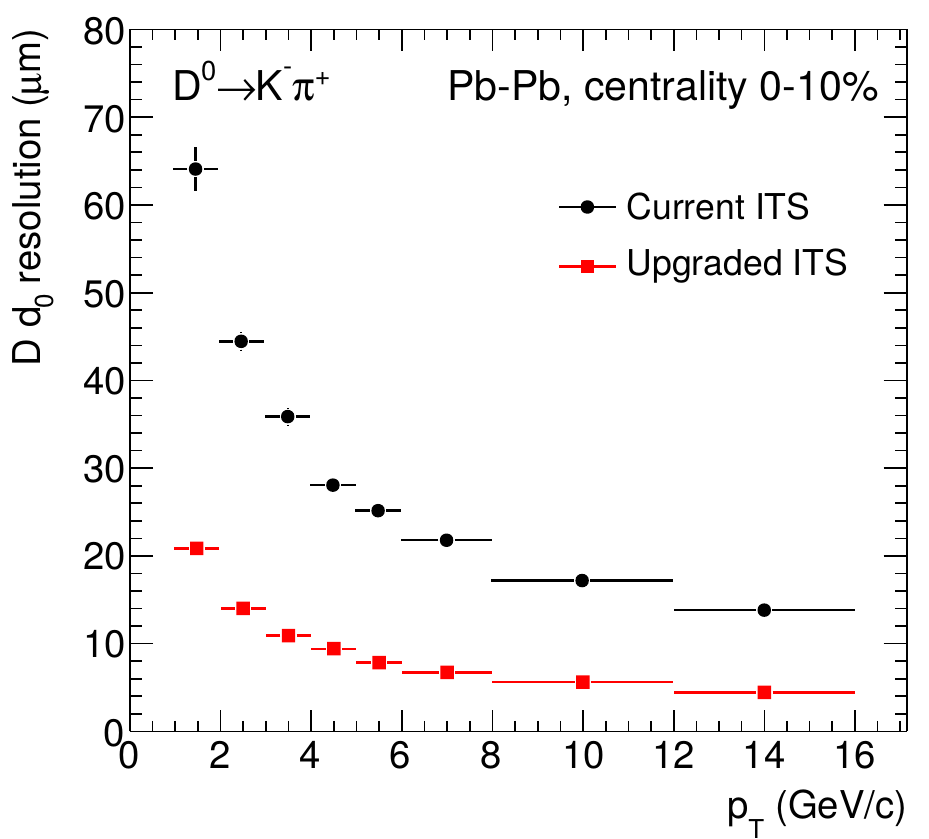
\includegraphics[scale=0.32]{figures/D0impres.png}}\quad
  {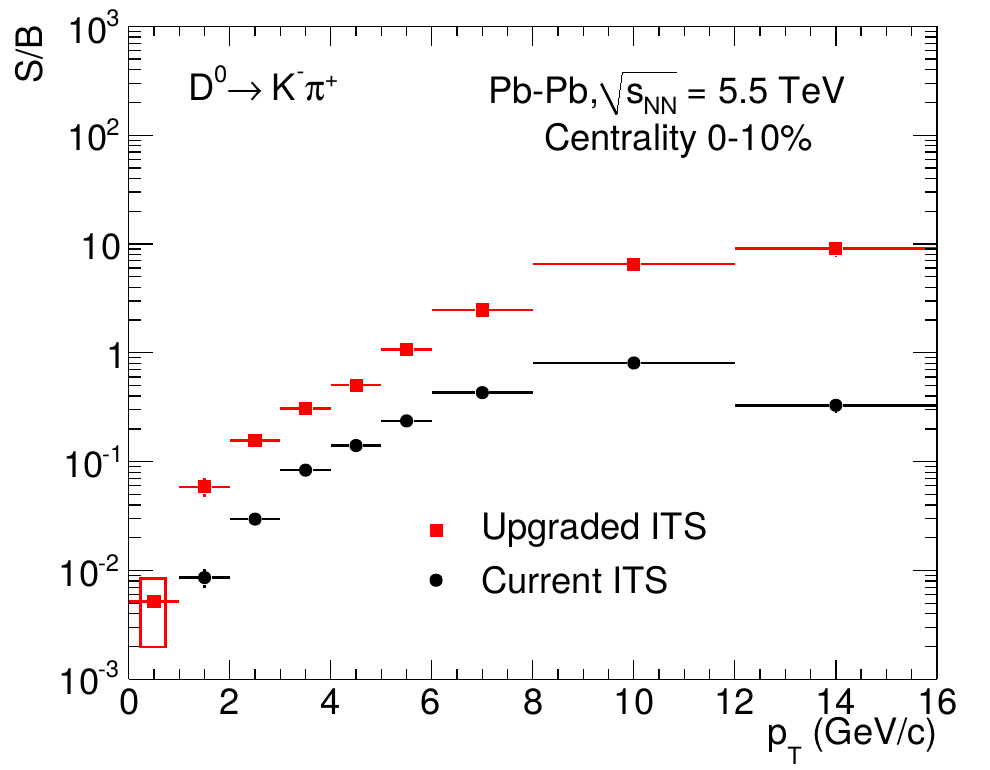
\includegraphics[scale=0.32]{figures/SoverB.png}}
  \caption{$D^0$ impact parameter resolution (upper panel) and $D^0$ signal-to noise ratio (lower panel) \cite{uptdr}.}
  \label{fig:d0stuff}
\end{figure}
\section{Online-Offline Computing System: O$^2$}
Mainly for the higher collision rate foreseen for Run3, but also for the increased number of readout channels, the data rate of the experiment will considerably increase after the upgrade, passing from the present value of about 25 GB/s to more than 1 TB/s. Almost the totality of this figure comes from the TPC, while the ITSU alone will provide 40 GB/s, that alone is more than the rate of all the detectors in the present configuration \cite{o2}. In order to deal with the new data rate, the DAQ, the HLT and the offline system will be replaced by a new Online-Offline integrated framework ($O^2$). The O$^2$ system will reduce the data volume online, in parallel with the data collection, without rejecting any event as with the trigger systems. In particular, the O$^2$ will perform a partial calibration and reconstruction online, substituting the original raw data with compressed data. The result is the production of \textit{Compressed Time Frames} (CTF), containing the processed data from all the active detectors for a period of time $\approx$ 20 ms. In particular, for the TPC and the ITS, the data are directly saved in cluster format. In addition, for the TPC, clusters not belonging to tracks or identified as background are rejected, allowing to compress the information to the maximum. From here on, CTFs are immutable and can be stored. Since this first reconstruction will be performed synchronously with the data acquisition, the O$^2$ facility will be equipped with hardware accelerators, such as \textit{Graphic Processing Units} (GPU) and \textit{Field Programmable Gate Arrays} (FPGA), to ensure sufficiently fast processing. Indeed, the first reconstruction can be performed with a high degree of parallelism because of the local and independent nature of the data. The following steps of the reconstruction are performed asynchronously, starting from the CTFs. Here an important role is played by the \textit{Grid}, the distributed computing system that connects the facilities of different institutes participating in the experiment \cite{tdrold}. A computing centre of the Grid is called \textit{Tier}: Tier-0 is the computing centre of CERN, Tier-1s are large regional centres and Tier-2s are small centres clustered around Tier-1s. For the data acquisition of Pb-Pb events, the O$^2$ facility will not be sufficient to process all the CTFs while performing the synchronous reconstruction. Indeed, only 2/3 of the asynchronous processes of reconstruction and calibration will be processed by the O$^2$ facility and the remaining 1/3 will be processed by Tier-0 and Tier-1s. The result of the second level asynchronous reconstruction is the production of \textit{Analysis Object Data} (AOD), which contain the final track parameters in a given vertex and for a given event. AOD are then analysed in dedicated \textit{High Performance Computing} (HPC) sites, called \textit{Analysis Facilities} (AF). AFs are capable of locally processing large data volumes: almost 5 PB in twelve hours.